\chapter{Specifikacija programske potpore}
		
	\section{Funkcionalni zahtjevi}			
			
			\noindent \textbf{Dionici:}
			
			\begin{packed_enum}
				
				\item Korisnik
				\begin{packed_enum}
					\item Anonimni korisnik
					\item Registrirani korisnik		
				\end{packed_enum}
				\item Administrator
				
			\end{packed_enum}
			
			\noindent \textbf{Aktori i njihovi funkcionalni zahtjevi:}
			
			
			\begin{packed_enum}
				\item  \underbar{anonimni korisnik (inicijator) može:}
				
				\begin{packed_enum}
					
					\item pridružiti se igri kao anoniman korisnik
					\begin{packed_enum}						
						\item  sustav mu dodjeljuje nadimak 				
					\end{packed_enum}
					
				\end{packed_enum}
			
				\item  \underbar{registrirani korisnik (inicijator) može:}
				
				\begin{packed_enum}
					
					\item unijeti nadimak i zaporku
					\item pratiti vlastitu statistiku u igri
					\item promijeniti izgled vozila u izborniku
					\item brisati svoj račun
					
				\end{packed_enum}
				\item  \underbar{administrator (inicijator) može:}
					\begin{packed_enum}
						\item uređivati liste mapa aktivnih unutar igre
						\item pretraživati korisnika po nadimku i vidjeti prikaz njegove statistike
						\item pretraživati najbolje igrače
					\end{packed_enum}
				
				\item  \underbar{baza podataka (sudionik) može:}
				\begin{packed_enum}
					\item pohraniti podatke o korisniku
				\end{packed_enum}

			\end{packed_enum}
			
			\eject 
			
			
				
			\subsection{Obrasci uporabe}
			
				
				\subsubsection{Opis obrazaca uporabe}
					

					\noindent \underbar{\textbf{UC1 - registracija}}
					\begin{packed_item}
	
						\item \textbf{Glavni sudionik: }Neregistriran korisnik
						\item  \textbf{Cilj:} Stvoriti korisnički račun
						\item  \textbf{Sudionici:} Baza podataka
						\item  \textbf{Preduvjet:} -
						\item  \textbf{Opis osnovnog tijeka:}
						
						\item[] \begin{packed_enum}
	
							    \item Korisnik odabire gumb za registraciju
    							\item Korisnik unosi potrebne podatke – nadimak i zaporku
    							\item Provjerava se ispravnost podataka
    							\item Podaci se spremaju u bazu podataka
   								 \item Korisnik je uspješno registriran 
						\end{packed_enum}
						
						\item  \textbf{Opis mogućih odstupanja:}
						
						\item[] \begin{packed_item}
	
							\item[2.b] Korisnik unosi već korištene podatke
							\item[] \begin{packed_enum}
								
								\item Korisnik prima obavijest da se podaci koriste
								\item Omogućava se ponovni pokušaj korisniku
								
							\end{packed_enum}
							
						\end{packed_item}
					\end{packed_item}

										\noindent \underbar{\textbf{UC2 - prijava u sustav}}
					\begin{packed_item}
	
						   \item \textbf{Glavni sudionik: } Registriran korisnik
						   \item  \textbf{Cilj:} Korištenje mogućnosti registriranog korisnika
						   \item  \textbf{Sudionici:} Baza podataka
				 	   	   \item  \textbf{Preduvjet:} Korisnik je registriran
							\item  \textbf{Opis osnovnog tijeka:}
	
					\item[] \begin{packed_enum}
		
							\item Korisnik odabira gumb "Prijava"
							\item Korisnik upisuje korisničko ime i zaporku
							\item Provjerava se ispravnost podataka
							\item Korisnik je uspješno prijavljen
				\end{packed_enum}
	
					\item  \textbf{Opis mogućih odstupanja:}
	
						\item[] \begin{packed_item}
		
						\item[2.b] 
						\item[] \begin{packed_enum}
			
									\item Korisnik nije registriran
								\item Korisnik je unio krive podatke 
			
								\end{packed_enum}
		
						\end{packed_item}
				\end{packed_item}		
					
										\noindent \underbar{\textbf{UC3 - pregled vlastite statistike}}
					\begin{packed_item}
	
						\item \textbf{Glavni sudionik: }Registrirani korisnik
						\item  \textbf{Cilj:} Praćenje broja odigranih rundi i statistika pobjeda
						\item  \textbf{Sudionici:} Baza podataka
						\item  \textbf{Preduvjet:} Korisnik je registriran(UC1)
						\item  \textbf{Opis osnovnog tijeka:}
						
						\item[] \begin{packed_enum}
	
							    \item Korisnik odabire gumb „Moj račun“
							    \item Korisnik odabire gumb "Prikaži moju statistiku"
    							\item Korisniku piše broj odigranih rundi i pobjeda
						\end{packed_enum}
					\end{packed_item}
				
										\noindent \underbar{\textbf{UC4 - pregled statistike drugih igrača}}
					\begin{packed_item}
						
						\item \textbf{Glavni sudionik: } Registrirani korisnik
						\item  \textbf{Cilj:} Mogućnost pregleda statistike drugih registriranih korisnika pretraživanjem po nadimku
						\item  \textbf{Sudionici:} Baza podataka
						\item  \textbf{Preduvjet:} Korisnik je registriran(UC1)
						\item  \textbf{Opis osnovnog tijeka:}
						
						\item[] \begin{packed_enum}
							
							\item Korisnik odabire gumb „Moj račun“
							\item Korisnik bira polje „Pretraži igrače“
							\item U odabrano polje korisnik upisuje nadimak željenog igrača
							\item Sustav izbacuje statistiku traženog igrača iz baze podataka							
						\end{packed_enum}
						
						\item  \textbf{Opis mogućih odstupanja:}
						
						\item[] \begin{packed_item}
							
							\item[5.d] Traženi korisnik je obrisao profil					
						\end{packed_item}
					\end{packed_item}
				
										\noindent \underbar{\textbf{UC5 - resetiranje statistike}}
					\begin{packed_item}
						
						\item \textbf{Glavni sudionik: } Registrirani korisnik
						\item  \textbf{Cilj:} Mogućnost resetiranje dosadašnje statistike
						\item  \textbf{Sudionici:} Baza podataka
						\item  \textbf{Preduvjet:} Korisnik je registriran(UC1)
						\item  \textbf{Opis osnovnog tijeka:}
						
						\item[] \begin{packed_enum}
							
							\item Korisnik odabire gumb „Moj Račun“
							\item Korisnik  odabire opciju "Resetiraj statistiku"
							\item Sustav nudi korisniku u skočnom prozoru mogućnost da odustane klikom na gumb "Odustani" ili da resetira statistiku klikom na gumb "Resetiraj" 
							\item Korisnikova statistika se u bazi podatak postavi na 0
						\end{packed_enum}
					\end{packed_item}
				
				
				    	\noindent \underbar{\textbf{UC6 - odjava}}
				    \begin{packed_item}
				    	
				    	\item \textbf{Glavni sudionik: } Registrirani korisnik
				    	\item  \textbf{Cilj:} Odjaviti se iz sustava
				    	\item  \textbf{Sudionici:} -
				    	\item  \textbf{Preduvjet:} Korisnik je prijavljen u sustav (UC3)
				    	\item  \textbf{Opis osnovnog tijeka:}
				    	
				    	\item[] \begin{packed_enum}
				    		
				    		\item Korisnik zahtjeva odjavu iz sustava odabirom gumba "Odjava" na početnoj stranici
				    		\item Sustav odjavljuje korisnika
				    		\item Prikazuje se početna stranica
				    	\end{packed_enum}
				    \end{packed_item}
						
					
										\noindent \underbar{\textbf{UC7 - promjena osobnih podataka}}
					\begin{packed_item}
	
						\item \textbf{Glavni sudionik: } Registrirani korisnik
						\item  \textbf{Cilj:} Mogućnost promijene zaporke
						\item  \textbf{Sudionici:} Baza podataka
						\item  \textbf{Preduvjet:} Korisnik je registriran
						\item  \textbf{Opis osnovnog tijeka:}
						
						\item[] \begin{packed_enum}
	
							    \item Korisnik odabire gumb „Moj račun“
    							\item Korisnik odabire opcije za promjenu zaporke
    							\item Korisnik upisuje novu zaporku
    							\item Korisnik sprema promjene
    							\item Baza podataka se ažurira
						\end{packed_enum}
						
						\item  \textbf{Opis mogućih odstupanja:}
						
						\item[] \begin{packed_item}
	
							\item[5.d] Korisnik je upisao novu zaporku, ali nije spremio promjene
							\item[] \begin{packed_enum}
								
								\item  Sustav obavještava korisnika da nije spremio prije izlaska iz izbornika
								
							\end{packed_enum}
							
						\end{packed_item}
					\end{packed_item}
					
										\noindent \underbar{\textbf{UC8 - promjena izgleda vozila}}
					\begin{packed_item}
	
						\item \textbf{Glavni sudionik: } Registrirani korisnik
						\item  \textbf{Cilj:} Mogućnost promjene izgleda vozila među dostupnima
						\item  \textbf{Sudionici:} Baza podataka
						\item  \textbf{Preduvjet:} Korisnik je registriran
						\item  \textbf{Opis osnovnog tijeka:}
						
						\item[] \begin{packed_enum}
	
							    \item Korisnik odabire gumb „Moj Račun“
    							\item Korisnik  odabire opciju "Odaberi novi izgled"
    							\item Korisniku se prikazuje lista otključanih izgleda koje mu dodjeljuje sustav ovisno o broju pobjeda
						\end{packed_enum}
					\end{packed_item}
				
									\noindent \underbar{\textbf{UC9 - brisanje korisničkog računa}}
					\begin{packed_item}
						
						\item \textbf{Glavni sudionik: } Registrirani korisnik
						\item  \textbf{Cilj:} Obrisati korisnički račun
						\item  \textbf{Sudionici:} Baza podataka
						\item  \textbf{Preduvjet:} Korisnik je registriran
						\item  \textbf{Opis osnovnog tijeka:}
						
						\item[] \begin{packed_enum}
							
							\item Korisnik odabire gumb „Moj Račun“
							\item Korisnik  odabire opciju „Obriši račun“
							\item Korisnički račun se briše iz baze podataka
						\end{packed_enum}
					\end{packed_item}
					
					
								\noindent \underbar{\textbf{UC10 - odabir akcije nakon smanjena zdravlja igrača na 0}}
					\begin{packed_item}
						
						\item \textbf{Glavni sudionik: } Korisnik
						\item  \textbf{Cilj:} Korisnik može odlučiti hoće li napustiti igru ili će se vratiti nakon što mu je zdravlje smanjeno na 0
						\item  \textbf{Sudionici:} -
						\item  \textbf{Preduvjet:} -
						\item  \textbf{Opis osnovnog tijeka:}
						
						\item[] \begin{packed_enum}
							
							\item Korisniku je zdravlje smanjeno na 0 te ga se izbacuje iz trenutno aktivne runde
							\item Korisniku se pojavljuje skočni prozor 
							\item Korisnik odabire jednu od ponuđenih opcija
							\item Ako odabere "Napusti" on izlazi iz aktivne igre
							\item Ako odabere "Povratak u igru" on se vraća u aktivnu rundu
						\end{packed_enum}
						
						\item  \textbf{Opis mogućih odstupanja:}
						
						\item[] \begin{packed_item}
							
							\item[5.b] 
							\item[] \begin{packed_enum}
								
								\item Ako je u trenutku povratka u igru igra završila, sustav odbija vratit korisnika u igru
								\item Ako se korisnik želi vratiti u igru, mora pričekati 30 sekundi od izbacivanja 
								
							\end{packed_enum}
							
						\end{packed_item}
					\end{packed_item}
				
				    				\noindent \underbar{\textbf{UC11 - komuniciranje između igrača}}
				    \begin{packed_item}
				    	
				    	\item \textbf{Glavni sudionik: } Korisnici(Registrirani, anonimni)
				    	\item  \textbf{Cilj:} Mogućnost komunikacije između igrača unutar runde
				    	\item  \textbf{Sudionici:} Korisnici
				    	\item  \textbf{Preduvjet:} -
				    	\item  \textbf{Opis osnovnog tijeka:} 
				    	
				    	\item[] \begin{packed_enum}
				    		
				    		\item Korisnik klikom miša odabire tekstno polje na ekranu
				    		\item Korisnik piše poruku i šalje ostalim igračima
				    	\end{packed_enum}
				    \end{packed_item}
			    
			    					\noindent \underbar{\textbf{UC12 - ulazak korisnika u rundu}}
			    	\begin{packed_item}
			    		
			    		\item \textbf{Glavni sudionik: } Korisnik (Registrirani, anonimni)
			    		\item  \textbf{Cilj:} Ulazak korisnika u rundu
			    		\item  \textbf{Sudionici:} Baza podataka
			    		\item  \textbf{Preduvjet:} -
			    		\item  \textbf{Opis osnovnog tijeka:}
			    		
			    		\item[] \begin{packed_enum}
			    			
			    			\item Korisnik odabire gumb "Igraj"
			    			\item Server korisniku dodjeljuje rundu u koju može ući
			    			\item Korisnik ulazi u rundu i igra
			    		\end{packed_enum}
			    	
		               \item  \textbf{Opis mogućih odstupanja:}
		    			
		    			\item[] \begin{packed_item}
		    				
		    				\item[2.b] 
		    				\item[] \begin{packed_enum}
		    					
		    					\item Korisnik mora čekati da mu server dodjeli rundu za igru jer server raspodjeljuje s obzirom na dosadašnji uspjeh korisnika 
		    					
		    				\end{packed_enum}
		    				
		    			\end{packed_item}
	    			\end{packed_item}
			    
			    
			   						\noindent \underbar{\textbf{UC13 - prijava administratora u sustav}}
			   		\begin{packed_item}
			   			
			   			\item \textbf{Glavni sudionik: } Administrator
			   			\item  \textbf{Cilj:} Korištenje administracijskih ovlasti
			   			\item  \textbf{Sudionici:} Baza podataka
			   			\item  \textbf{Preduvjet:} Postojanje administratora 
			   			\item  \textbf{Opis osnovnog tijeka:}
			   			
			   			\item[] \begin{packed_enum}
			   				
			   				\item Administrator odabira gumb "Prijava administratora"
			   				\item Administrator upisuje ime i zaporku
			   				\item Provjerava se ispravnost podataka
			   				\item Administrator je uspješno prijavljen
			   			\end{packed_enum}
			   			
			   			\item  \textbf{Opis mogućih odstupanja:}
			   			
			   			\item[] \begin{packed_item}
			   				
			   				\item[2.b] 
			   				\item[] \begin{packed_enum}
			   					
			   					\item Ne postoji administrator s upisanim imenom
			   					\item Postoji ime administratora, ali je pogrešna zaporka
			   					
			   				\end{packed_enum}
			   				
			   			\end{packed_item}
			   		\end{packed_item}	
						
					
										\noindent \underbar{\textbf{UC14 - zabranjivanje pristupa korisniku}}
					\begin{packed_item}
	
						\item \textbf{Glavni sudionik: } Administrator
						\item  \textbf{Cilj:} Zabraniti korisnicima pristup igri
						\item  \textbf{Sudionici:} -
						\item  \textbf{Preduvjet:} -
						\item  \textbf{Opis osnovnog tijeka:}
						
						\item[] \begin{packed_enum}
	
							    \item Administrator pronalazi korisnika kojem želi zabraniti pristup
    							\item Administrator bira opciju "Blokiraj korisnika"
    							\item Administrator zabrani pristup korisniku trajno ili privremeno
						\end{packed_enum}
					\end{packed_item}
					
					
										\noindent \underbar{\textbf{UC15 - dodjela administratorskih ovlasti}}
					\begin{packed_item}
	
						\item \textbf{Glavni sudionik: } Administrator
						\item  \textbf{Cilj:} Dodavanje novog administratora u sustav
						\item  \textbf{Sudionici:} Baza podataka
						\item  \textbf{Preduvjet:} -
						\item  \textbf{Opis osnovnog tijeka:}
						
						\item[] \begin{packed_enum}
	
							    \item Administrator odabire gumb "Dodaj novog administratora"
    							\item Administrator u polje upisuje ime i zaporku
 								\item Administrator dodaje novog administratora
						\end{packed_enum}
						
						\item  \textbf{Opis mogućih odstupanja:}
						
						\item[] \begin{packed_item}
	
							\item[2.b] 
							\item[] \begin{packed_enum}
								
								\item U sustavu postoji administrator s istim imenom
								
							\end{packed_enum}
							
						\end{packed_item}
					\end{packed_item}
					
										\noindent \underbar{\textbf{UC16 - dodjela liste mape}}
					\begin{packed_item}
	
						\item \textbf{Glavni sudionik: } Administrator
						\item  \textbf{Cilj:} Odrediti liste mape koje će biti aktivne unutar igre
						\item  \textbf{Sudionici:} Baza podataka
						\item  \textbf{Preduvjet:} Nema igara u tijeku
						\item  \textbf{Opis osnovnog tijeka:}
						
						\item[] \begin{packed_enum}
	
							    \item Administrator bira opciju "Dodjela liste mapa"
    							\item Administrator odabere liste mape koje će biti aktivne unutar same igre
						\end{packed_enum}
						
						\item  \textbf{Opis mogućih odstupanja:}
						
						\item[] \begin{packed_item}
	
							\item[2.b] 
							\item[] \begin{packed_enum}
								
								\item  Postoje igre u tijeku te administrator ne može dodijeliti liste mapa
								\item  Igrači moraju pričekati da lista mapa bude dodijeljena
								
							\end{packed_enum}
							
						\end{packed_item}
					\end{packed_item}
					
										\noindent \underbar{\textbf{UC17 - pretraga najboljih igrača}}
					\begin{packed_item}
	
						\item \textbf{Glavni sudionik: } Administrator
						\item  \textbf{Cilj:} Pronaći igrače sa najviše ostvarenih bodova
						\item  \textbf{Sudionici:} Baza podataka
						\item  \textbf{Preduvjet:} -
						\item  \textbf{Opis osnovnog tijeka:}
						
						\item[] \begin{packed_enum}
	
							    \item Administrator odabire opcije "Pretraga igrača"
    							\item Administrator odabire zatim opciju "Pretraži po rezultatu"
    							\item Administrator u tekstno polje upisuje broj korisnika koje pretražuje
    							\item Administrator odabire korisnika i ima uvid u dosadašnji uspjeh
						\end{packed_enum}
					\end{packed_item}
				
										\noindent \underbar{\textbf{UC18 - brisanje korisnika}}
					\begin{packed_item}
						
						\item \textbf{Glavni sudionik: } Administrator
						\item  \textbf{Cilj:} Obrisati korisnika
						\item  \textbf{Sudionici:} Baza podataka
						\item  \textbf{Preduvjet:} Korisnik je registriran
						\item  \textbf{Opis osnovnog tijeka:}
						
						\item[] \begin{packed_enum}
							
							\item Administrator odabire opcije "Uklanjanje korisnika"
							\item Administrator u tekstno polje upisuje ime korisnika
							\item Administrator pronalazi korisnika, uklanja ga i njegove podatke iz baze podataka
						\end{packed_enum}
					\end{packed_item}	
				
			    \newpage
				\subsubsection{Dijagrami obrazaca uporabe}
				
				\begin{figure}[h]
					\centering
					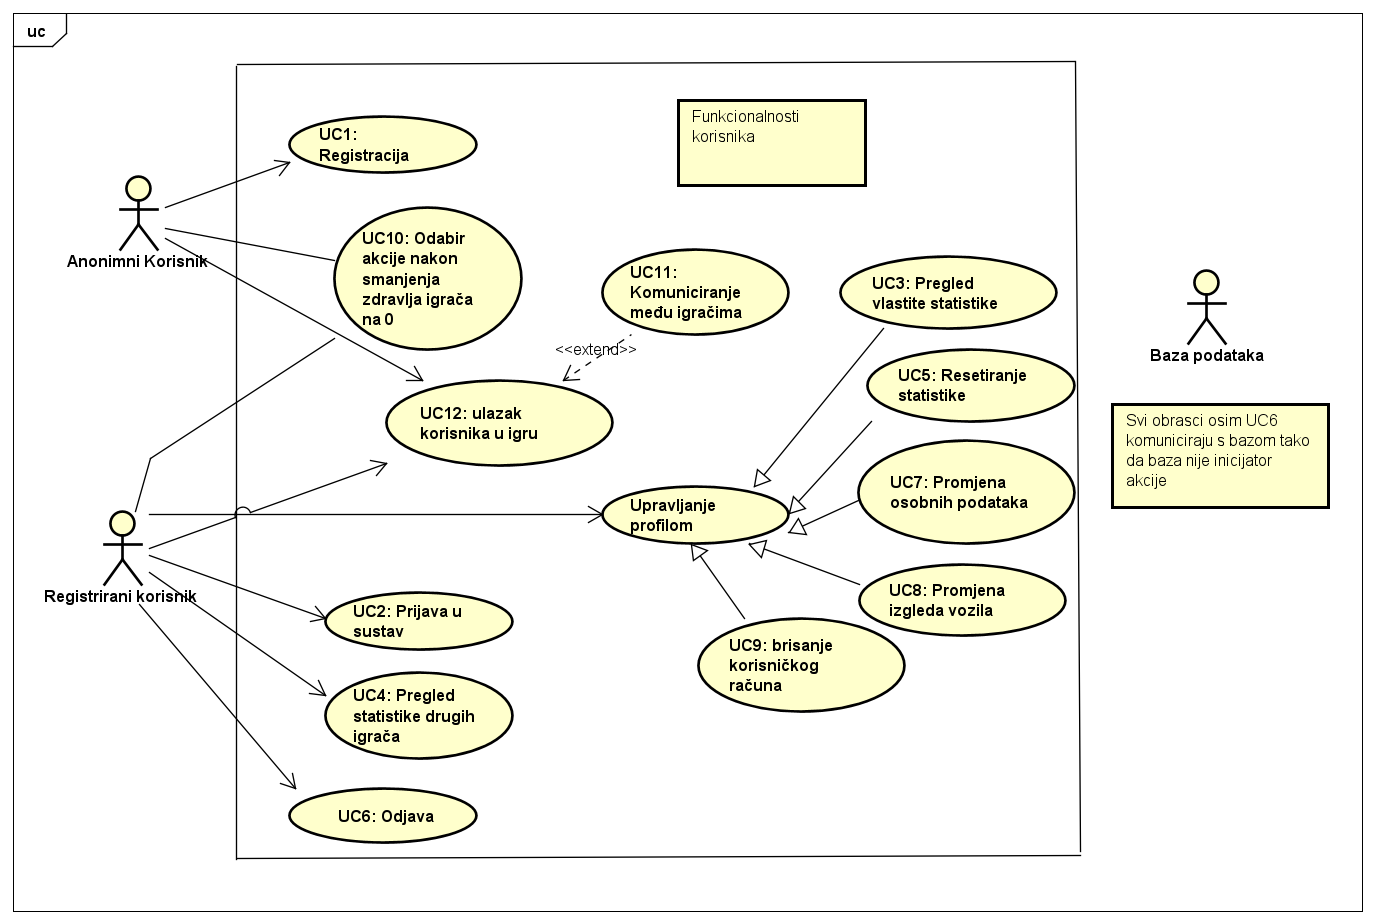
\includegraphics[width=18.5cm,height=14.5cm]{useCaseDiagram1}
					\caption{Dijagram obrazaca uporabe, funkcionalnosti korisnika}
					\label{fig:uc1}
				\end{figure}
			
			    \begin{figure}[h]
			    	\centering
			    	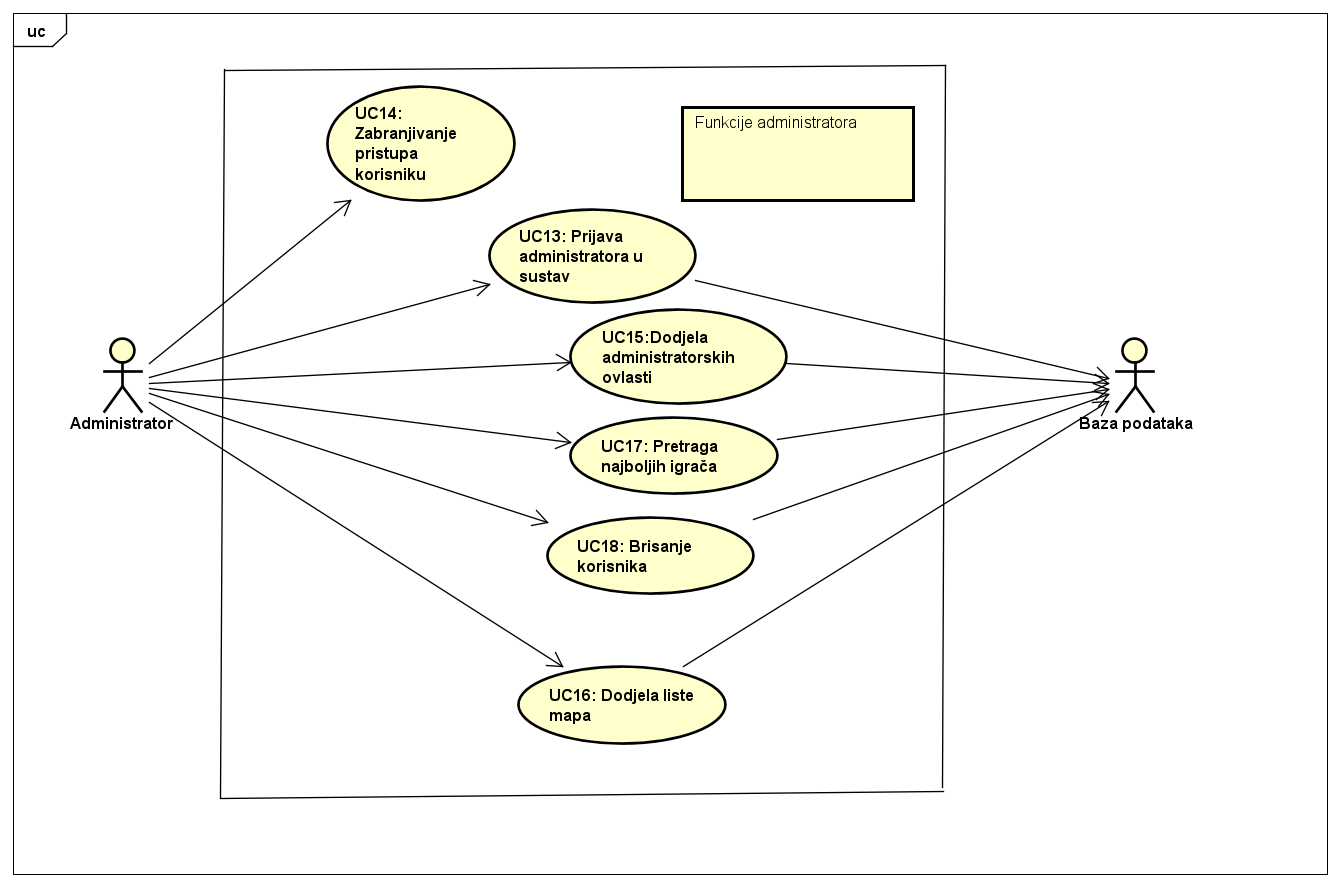
\includegraphics[width=18.5cm,height=14.5cm]{useCaseDiagram2}
			    	\caption{Dijagram obrazaca uporabe, funkcionalnosti administratora}
			    	\label{fig:uc2}
			    \end{figure}
					
				\eject		
				
				
				\newpage
			\subsection{Sekvencijski dijagrami}

			
				\textbf{\textit{Obrazac uporabe UC12 - ulazak korisnika u rundu}}\\
				\textit Korisnik želi ući u igru te odabire gumb igraj na web pregledniku. Zahtjev se šalje prema serveru. Korisnik ako je registriran ima svoju dosadašnju statistiku u bazi podataka te se prema njoj traži runda u kojoj su igrači slične razine iskustva. Ukoliko se igrača ne može svrstati u rundu u trenutku zahtjev će se slati opet dok server ne pronađe rundu u koju može korisnik ući.
				Ako u igru pak želi ući anonimni korisnik, on ima fiksan relativni učinak dodijeljen od implementiranog ELO algoritma te će se njega rasporediti u rundu s ostalim anonimnim korisnicima.\\
				
				\begin{figure}[h]
					\centering
					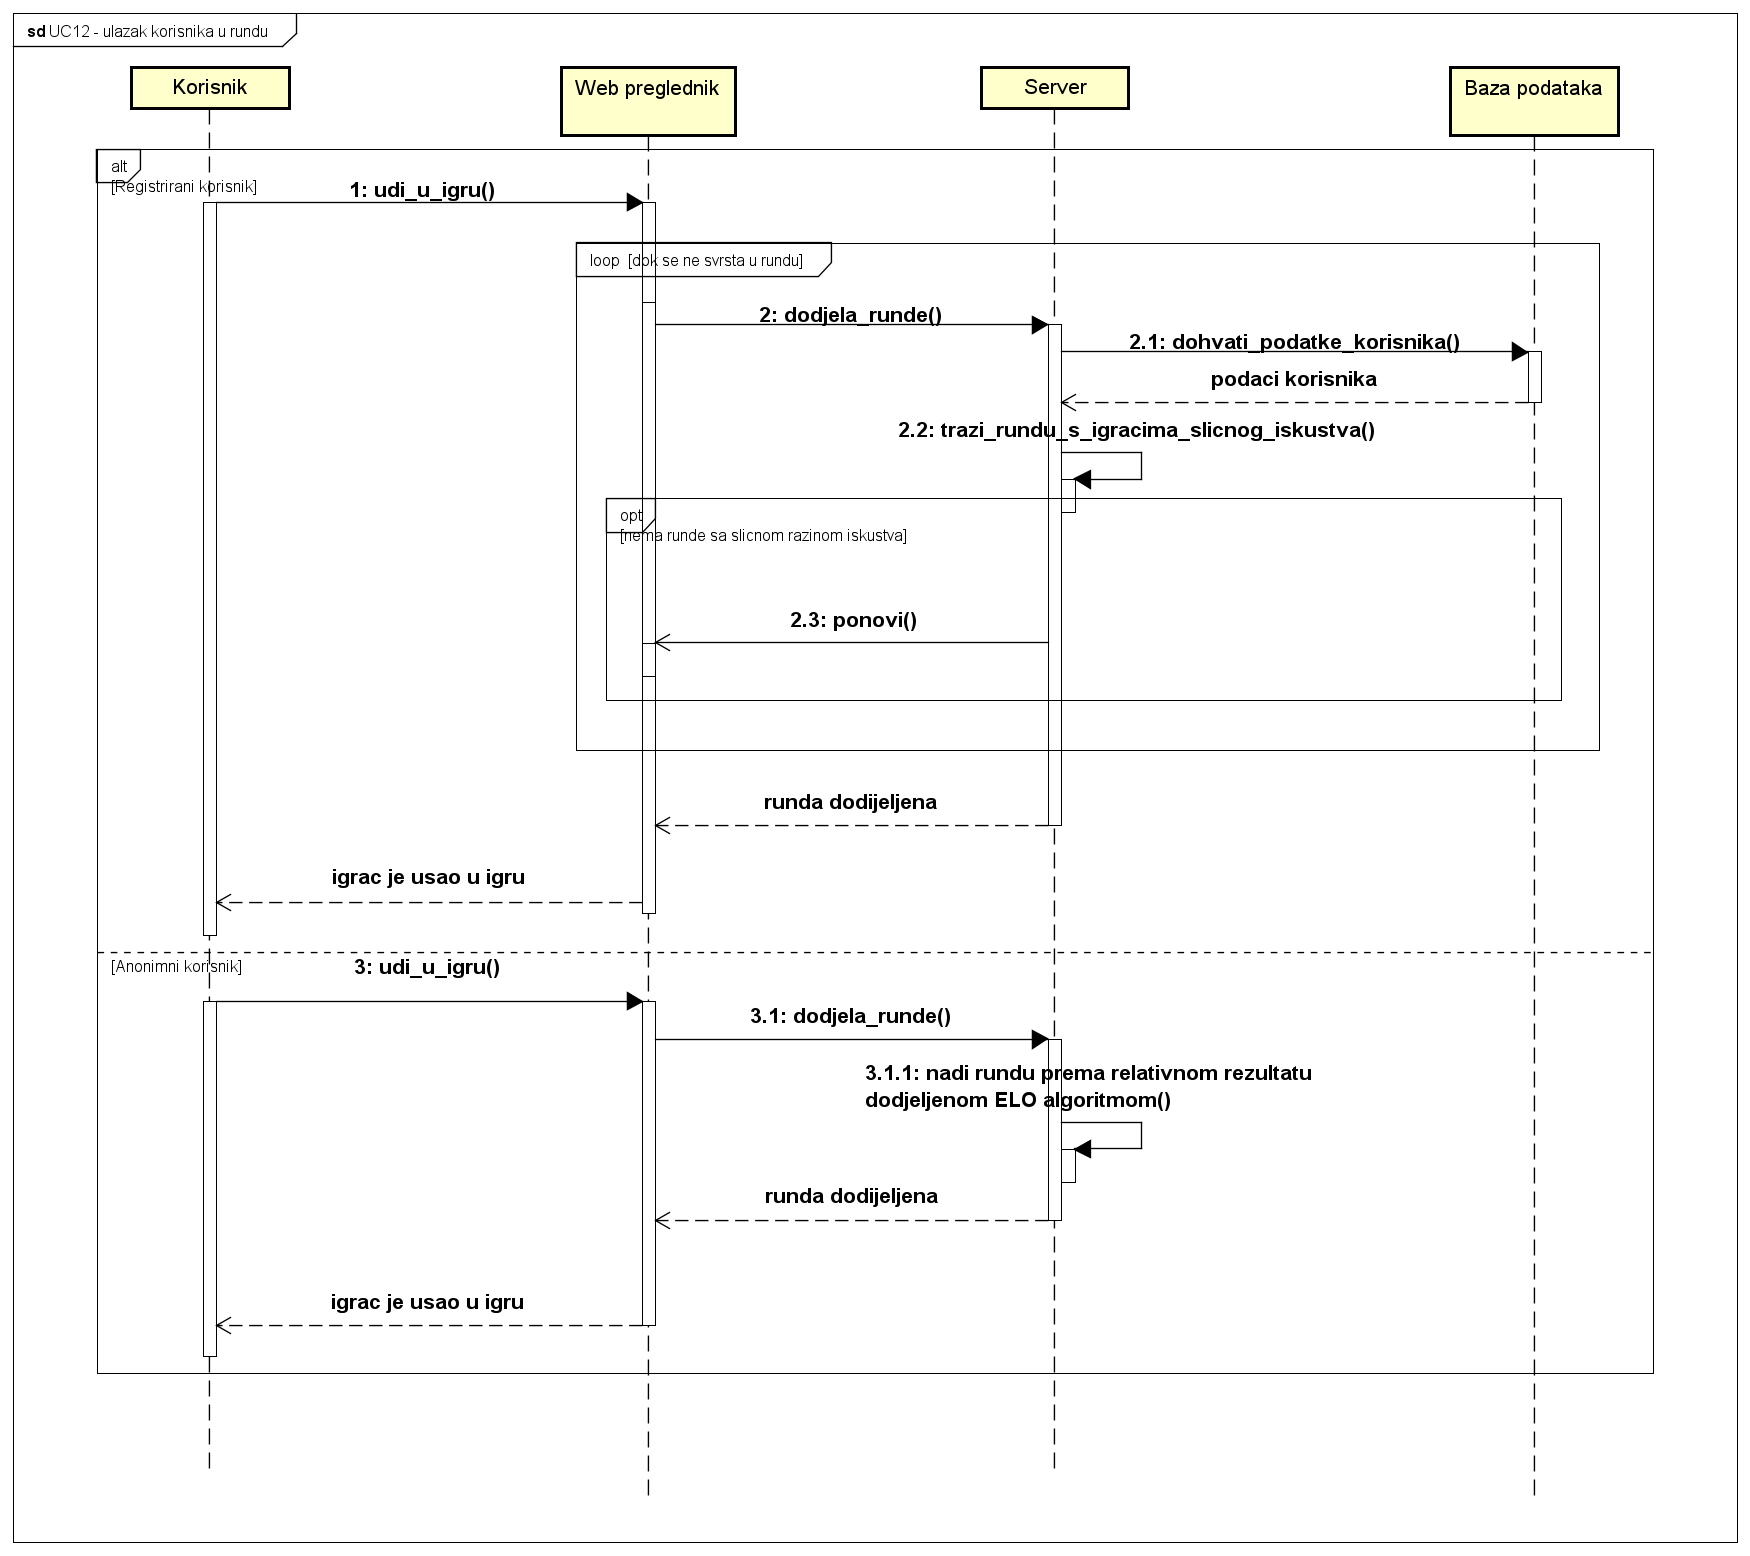
\includegraphics[width=18.5cm,height=15cm]{sequenceDiagram}
					\caption{Sekvencijski dijagram za UC12}
					\label{fig:uc12}
				\end{figure}
				
				\newpage
				\textbf{\textit{Obrazac uporabe UC3 - pregled vlastite statistike}}\\
				\textit Korisniku se pritiskom na gumb "Moj račun", kojeg vidi na web pregledniku, otvara izbornik gdje ima mogućnost odabrati gumb "Prikaži moju statistiku". Web preglednik će zahtjev za tom akcijom poslati serveru koji taj zahtjev šalje direktno bazi podataka. Baza podataka zatim pronađe statistiku traženog igrača i vraća podatke serveru. Server zatim šalje podatke web pregledniku, a na samom web pregledniku korisnik zatim može vidjeti svoju najnoviju statistiku.\\
				
				\begin{figure}[h]
					\centering
					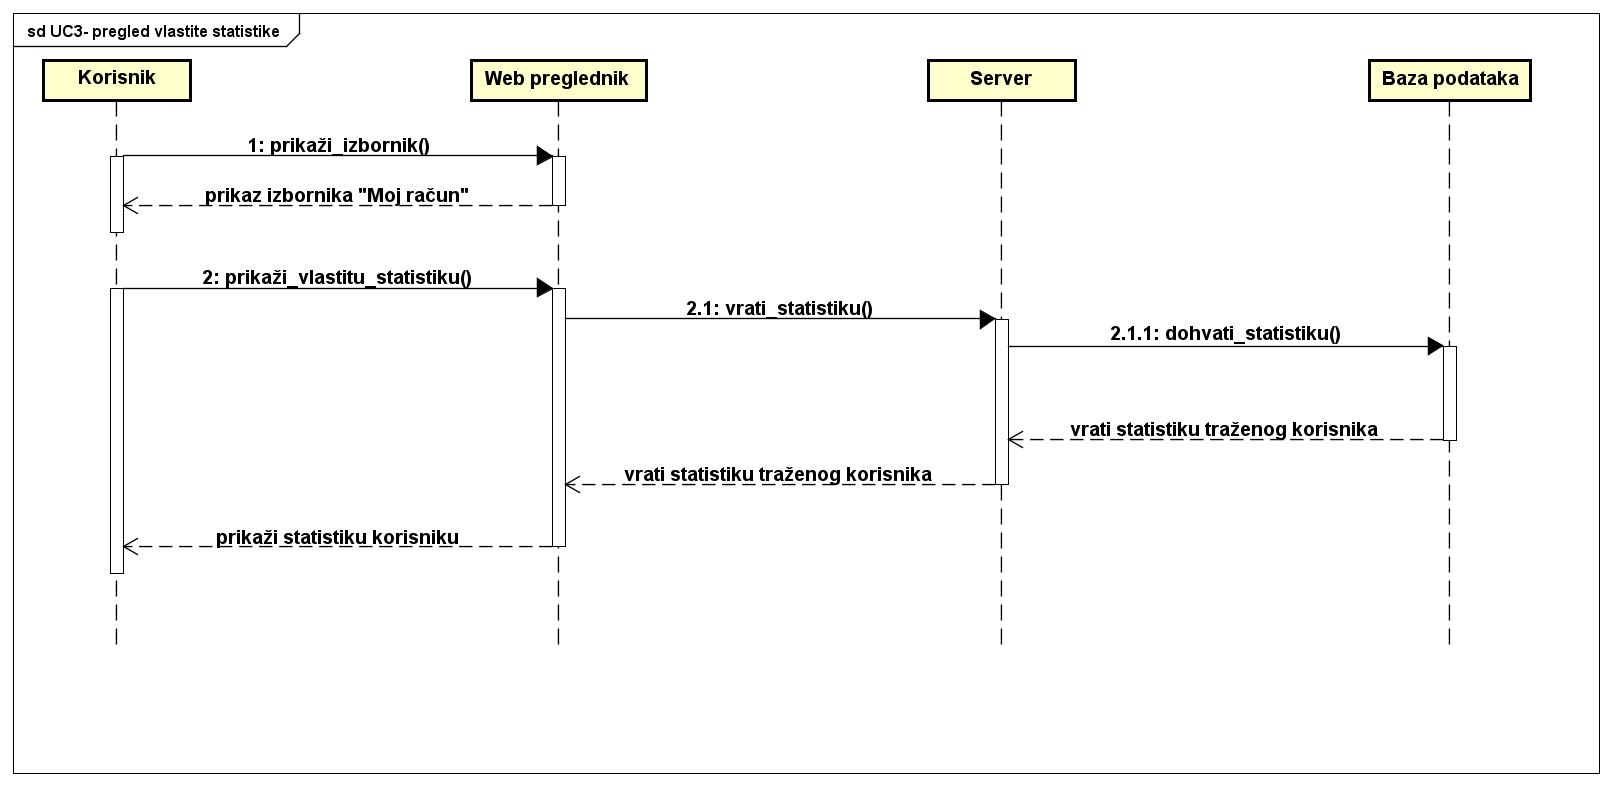
\includegraphics[width=17cm,height=12cm]{sequenceDiagram2}
					\caption{Sekvencijski dijagram za UC3}
					\label{fig:uc3}
				\end{figure}
				

				\newpage
		\section{Ostali zahtjevi}

			 \begin{enumerate}
			 	\item Prilikom registracije sustav mora upozoriti korisnika da je korisničko ime već zauzeto.
			 	\item Sustav mora podržati istodobno barem jednog administratora i barem 4 redovna korisnika.
			 	\item Sustav mora biti jednostavan za korištenje, a sučelje mora biti jasno i intuitivno.
			 	\item Sustav mora podržati hrvatske dijakritičke znakove za korisnička imena i prilikom komunikacije u prozoru za poruke.
			 	\item Sustav se temelji na HTML-u, CSS-u i JavaScriptu na korisničkoj strani te Node.js-u s express-om na serverskoj strani. 
			 	\item Koristi protokol HTTPS za komunikaciju između servera i preglednika weba.
			 	\item Sustav podržava do 50 korisnika.
			 	\item Korisnički podaci moraju biti zaštićeni nekim od algoritama enkripcije.
			 	\item Traženje nove igre ne smije trajati dulje od 5 minuta.
			 	\item Sve naknadne nadogradnje sustava ne smiju narušavati prijašnje funkcionalnosti sustava.
			 	\item Igrici se može pristupiti HTTPS-om iz javne mreže.
			 \end{enumerate}
			 
			 
	